\PassOptionsToPackage{unicode=true}{hyperref} % options for packages loaded elsewhere
\PassOptionsToPackage{hyphens}{url}
%
\documentclass[letterpaper]{article}
\usepackage{lmodern}
\usepackage{xcolor}
\usepackage{fontspec}
\usepackage{minted}
\usepackage{amssymb,amsmath}
\usepackage{ifxetex,ifluatex}
\usepackage[margin=1in]{geometry}
\usepackage{fixltx2e} % provides \textsubscript
\ifnum 0\ifxetex 1\fi\ifluatex 1\fi=0 % if pdftex
  \usepackage[T1]{fontenc}
  \usepackage[utf8]{inputenc}
  \usepackage{textcomp} % provides euro and other symbols
\else % if luatex or xelatex
  \usepackage{unicode-math}
  \defaultfontfeatures{Ligatures=TeX,Scale=MatchLowercase}
\fi
% use upquote if available, for straight quotes in verbatim environments
\IfFileExists{upquote.sty}{\usepackage{upquote}}{}
% use microtype if available
\IfFileExists{microtype.sty}{%
\usepackage[]{microtype}
\UseMicrotypeSet[protrusion]{basicmath} % disable protrusion for tt fonts
}{}
\IfFileExists{parskip.sty}{%
\usepackage{parskip}
}{% else
\setlength{\parindent}{0pt}
\setlength{\parskip}{6pt plus 2pt minus 1pt}
}
\usepackage{hyperref}
\hypersetup{
            pdfborder={0 0 0},
            breaklinks=true}
\urlstyle{same}  % don't use monospace font for urls
\usepackage{longtable,booktabs}
% Fix footnotes in tables (requires footnote package)
\IfFileExists{footnote.sty}{\usepackage{footnote}\makesavenoteenv{longtable}}{}
\usepackage{graphicx,grffile}
\makeatletter
\def\maxwidth{\ifdim\Gin@nat@width>\linewidth\linewidth\else\Gin@nat@width\fi}
\def\maxheight{\ifdim\Gin@nat@height>\textheight\textheight\else\Gin@nat@height\fi}
\makeatother
% Scale images if necessary, so that they will not overflow the page
% margins by default, and it is still possible to overwrite the defaults
% using explicit options in \includegraphics[width, height, ...]{}
\setkeys{Gin}{width=\maxwidth,height=\maxheight,keepaspectratio}
\setlength{\emergencystretch}{3em}  % prevent overfull lines
\providecommand{\tightlist}{%
  \setlength{\itemsep}{0pt}\setlength{\parskip}{0pt}}
\setcounter{secnumdepth}{0}
% Redefines (sub)paragraphs to behave more like sections
\ifx\paragraph\undefined\else
\let\oldparagraph\paragraph
\renewcommand{\paragraph}[1]{\oldparagraph{#1}\mbox{}}
\fi
\ifx\subparagraph\undefined\else
\let\oldsubparagraph\subparagraph
\renewcommand{\subparagraph}[1]{\oldsubparagraph{#1}\mbox{}}
\fi

% set default figure placement to htbp
\makeatletter
\def\fps@figure{htbp}
\makeatother


\date{}

\begin{document}

\hypertarget{bgp-extrapolator-propagation-design}{%
\section{BGP Extrapolator Propagation Design
}\label{bgp-extrapolator-propagation-design}}

\hypertarget{objective}{%
\subsection{Objective}\label{objective}}

The objectives of the extrapolator are to estimate the local routing
information base (RIB) of every AS in the internet and also to simulate
different routing policies for routing security experiments.

\hypertarget{introduction}{%
\subsection{Introduction}\label{introduction}}

The BGP extrapolator propagates route announcements based on the
well-known Gao-Rexford, or valley-free routing model. This model assumes
that ASes always prefer announcements received from customers over
announcements received from peers, which are further preferred over ones
received from providers. Additionally, an AS would never announce a
route received from one provider to another provider, since it would end
up paying twice to route traffic that was not its own or its customer's.
In cases where an announcement for the same prefix is received from
multiple neighbors with the same relation, an AS prefers the
announcement with the shortest AS\_PATH.

Intuitively, this model makes sense because an AS will pay for traffic
sent to its providers, but not for traffic sent to peers, and it will
get paid for traffic sent to customers. If the only available path is
via a provider, an AS will want to announce that route to all of its
customers, however, it would never announce that route to its other
providers. Any announcement received from one of its customers is
forwarded to everyone, including other customers, peers, and providers.
This is in-line with the business incentives of an AS.

Below is a high-level overview of the algorithm.

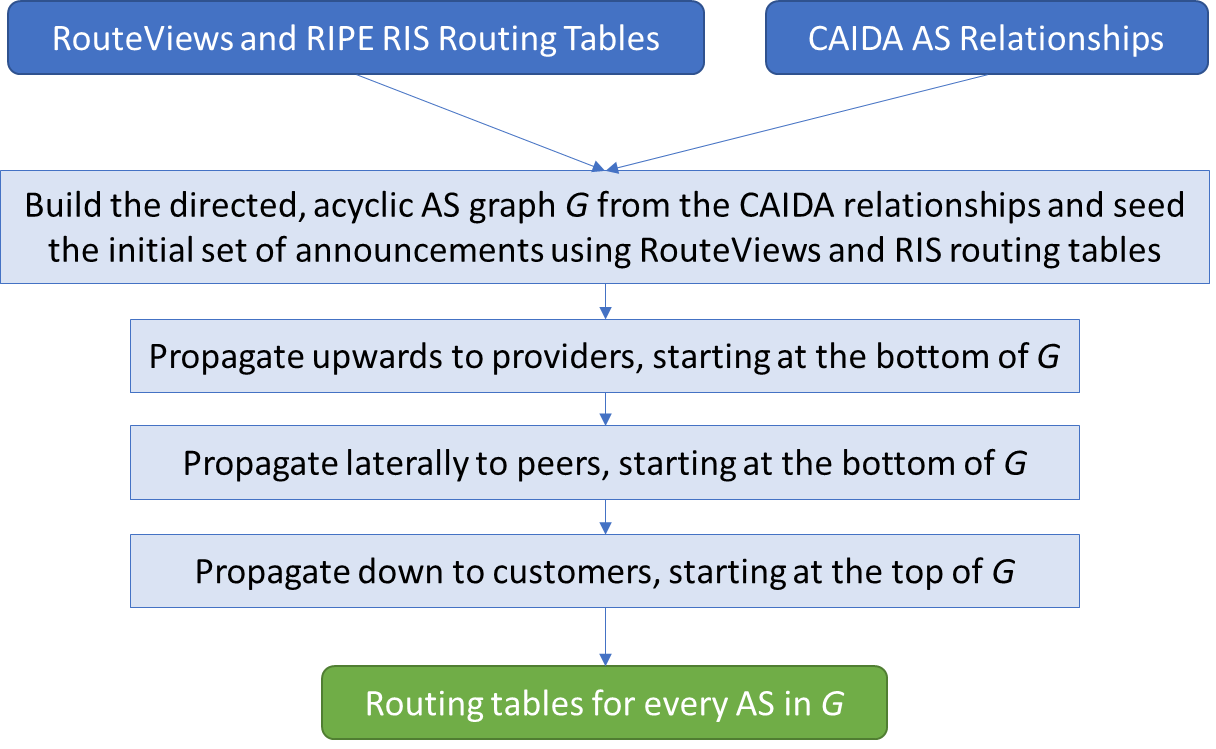
\includegraphics[width=6.1913in,height=3.81342in]{.//media/image1.png}

\hypertarget{steps}{%
\subsection{Steps}\label{steps}}

\textbf{Building the AS Graph}

Construct an AS Graph from the CAIDA AS Relationship data. Note that the
CAIDA topology does not include any sibling relationships. In the
topology, there are several strongly connected components where, for
example, AS \emph{x} is a customer of AS \emph{y} and \emph{y} is also a
customer of \emph{x}. A strongly connected component is collapsed into a
single AS, since it behaves like single AS and all members of the
component have equivalent RIBs.

\textbf{Seeding}

For every MRT announcement, emplace that announcement into the AS Graph
at the ASes on the AS\_PATH. When an AS is prepended multiple times to
the path, the path length is incremented but the other attributes of the
announcement stay the same.

Announcements containing loops are omitted from this process.

Other deviations from normal BGP such as path poisoning, or possible
strange types of path prepending are not accounted for, so these could
result in announcements being placed where they should not be.

When using MRT traces to populate the AS graph, sometimes different MRTs
contain different announcements depending on when they were created.  Since
paths in the internet are generally stable, we give preference to the path with
the oldest timestamp in cases where paths conflict. This method will be
incorrect when a path legitimately changes, however, it filters out
inconsistencies caused by events such as an MRT being created before the RIB
has stabilized after a route refresh since the recently refreshed routes will
have a newer timestamp.

\textbf{Gao Rexford Propagation and Tiebreaking}

The Extrapolator propagates up, laterally, and then down the AS Graph based on
the following path selection criteria. The attribute at the top of the table
has the highest priority, ties are broken by comparing attributes, starting at
the top of this list. Paths in the internet are generally stable,
so we give older announcements higher priority than newer ones.

\begin{enumerate}
  \item AS Relationship
  \item Shortest Path
  \item Oldest
  \item Random
\end{enumerate}

In contrast to real BGP shown below, we do not store information beyond the
path length, so we omit the lower three steps.

\begin{enumerate}
  \item AS Relationship
  \item Shortest Path
  \item Lowest Origin Type (e.g. IGP over EGP)
  \item MED and other tiebreakers
  \item Lowest BGP ID
\end{enumerate}

Stub ASes, which are ASes that have no customers or peers, are omitted
from the propagation, since their routing tables will be identical to
their providers, except for the additional hop to get to that provider.
Propagation is done in batches of prefixes to save on memory.

The Extrapolator, by default, will only propagate announcements from
multi-homed ASes when none of their providers have received that announcement.
For example, a multi-homed AS which is also a collector may report a route with
itself as the origin, and in this case, it should be propagated according to
the regular propagation rules. If, however, another collector reported a path
for that same prefix and multi-homed origin through one of its providers, then
the multi-homed origin does not send that announcement to all of its providers.
This is to accommodate for common primary-backup configurations where an AS
prefers one of its providers but maintains multiple providers for redundancy. 

The propagation logic does not treat IXPs differently than normal
ASes, even though it is known that they often do not use Gao Rexford
export policies.

\hypertarget{constraints}{%
\subsection{Compute Resources Constraints}\label{constraints}}

Must use \textless{} 80 GB RAM, 800 GB disk.

\hypertarget{models}{%
\subsection{Models}\label{models}}


\textbf{Priority}

The priority attribute is used internally to track the relationship and path
length of an announcement. The information is encoded into an integer, where
the first two decimal digits are used for the path length and the third decimal
is used for the relationship. 

Examples:

\begin{longtable}[]{@{}r|l@{}}
\toprule
\textbf{Priority} & \textbf{Explanation} \tabularnewline
\endhead
\midrule
300 & The highest priority value, a prefix originated at this AS. \tabularnewline
299 & Announcement received from a customer (path length of one). \tabularnewline
298 & Announcement received from a customer's customer (path length of two). \tabularnewline
198 & Announcement received from a peer (path length of two). \tabularnewline
97 & Announcement received from a provider (path length of three). \tabularnewline
\bottomrule
\end{longtable}

\textcolor{purple}{
\textbf{Proposed redesign}
  The priority attribute is a struct with four 8-bit fields carrying information
  relevant to the best-path selection process. This struct can be casted to an
  unsigned 32 bit integer to efficiently compare the priority of two different
  announcements. Reserved fields can be used to add other elements to the
  decision process, for example, security attributes like ROA validity.
}

\begin{minted}{C++}
struct Priority {
  // Little-endian assumed
  uint8_t reserved1;
  uint8_t path_length; // Lower precedence
  uint8_t reserved2;
  uint8_t relationship; // Highest precedence
};
\end{minted}

\textbf{Results Schema}

\begin{longtable}[]{@{}l|l@{}}
\toprule
\textbf{Column} & \textbf{Type}\tabularnewline
\endhead
\midrule
ASN & Bigint\tabularnewline
Prefix & CIDR\tabularnewline
Origin & Bigint\tabularnewline
Received\_from\_ASN & Bigint\tabularnewline
\bottomrule
\end{longtable}

\textbf{Input Schema}

\begin{longtable}[]{@{}l|l@{}}
\toprule
\textbf{Column} & \textbf{Type}\tabularnewline
\endhead
\midrule
Origin & Bigint\tabularnewline
Prefix & CIDR\tabularnewline
AS\_PATH & Bigint{[}{]}\tabularnewline
Time & Bigint\tabularnewline
\bottomrule
\end{longtable}

\textbf{Inverse Results Schema}

\begin{longtable}[]{@{}l|l@{}}
\toprule
\textbf{Column} & \textbf{Type}\tabularnewline
\endhead
\midrule
ASN & Bigint\tabularnewline
Prefix & CIDR\tabularnewline
Origin & Bigint\tabularnewline
\bottomrule
\end{longtable}

\textbf{Stubs Schema}

\begin{longtable}[]{@{}l|l@{}}
\toprule
\textbf{Column} & \textbf{Type}\tabularnewline
\endhead
\midrule
stub\_asn & Bigint\tabularnewline
parent\_asn & Bigint\tabularnewline
\bottomrule
\end{longtable}

\textbf{\\
}

\textbf{Announcement and AS struct}

\begin{longtable}[]{@{}l@{}}
\toprule
\textbf{Announcement}\tabularnewline
\midrule
\endhead
\begin{minipage}[t]{0.97\columnwidth}\raggedright
\begin{minted}{C++}
Prefix<> prefix;            // encoded with subnet mask
uint32_t origin;            // origin ASN
uint32_t priority;          // priority assigned based upon path length and AS relation
uint32_t received_from_asn; // ASN that sent the ann
bool from_monitor = false;  // flag for seeded ann from MRT announcements
int64_t tstamp;             // timestamp from mrt file

\end{minted}
\end{minipage}\tabularnewline
\bottomrule
\end{longtable}

\begin{longtable}[]{@{}l@{}}
\toprule
\textbf{BaseAS}\tabularnewline
\midrule
\endhead
\begin{minipage}[t]{0.97\columnwidth}\raggedright
\begin{minted}{C++}
uint32_t asn;     
int rank;                         // Rank in ASGraph hierarchy for propagation 
std::minstd_rand ran_bool;        // Random Number Generator
std::vector<AnnouncementType> *incoming_announcements;
std::map<Prefix<>, AnnouncementType> *all_anns;    // Maps of all announcements stored
std::map<Prefix<>, AnnouncementType> *depref_anns;

std::set<uint32_t> *providers; 
std::set<uint32_t> *peers; 
std::set<uint32_t> *customers; 

std::map<std::pair<Prefix<>, uint32_t>,std::set<uint32_t>*> *inverse_results; 

// If this AS represents multiple ASes, its "members" are listed here (Supernodes)  
std::vector<uint32_t> *member_ases;
// Assigned and used in Tarjan's algorithm
int index;
int lowlink;
bool onStack;
bool visited;      
\end{minted}
\strut
\end{minipage}\tabularnewline
\bottomrule
\end{longtable}

\end{document}
